\chapter{Vida Decision Support System} \label{ch:vida}


\section{\hlc[cyan]{Chapter Purpose \& Structure}}

Like Chapter \ref{ch:mangroves}, the case study detailed in this chapter is in service to multiple objectives. First, it seeks to address Research Question 2: ``What are the sustainability benefits of collaborative development of \acp{dss} using the \acf{evdt} Modeling Framework in complex \acf{sets}?" It accomplishes this by providing a case study demonstration of Research Deliverables 2a, 2b, and 2c: 

	\begin{enumerate}[label=\emph{\alph*},itemsep=0pt,parsep=0pt]
		\item{System architecture analyses of each of the case studies} 
		\item{Development of an \ac{evdt}-based \acf{dss} for each of the case studies} 
		\item{An interview-based assessment of the development process and usefulness of each \ac{dss}} 
	\end{enumerate}
	
Through these deliverables, this chapter serves as a demonstration of the \ac{evdt} Framework. The structure of this chapter thus mirrors the components of the framework laid out in Section \ref{sec:framework}. It starts by walking through the steps of the \acf{saf} as applied to this case study in Section \ref{sec:vida-saf}. These are separated into the methodology used for each step of the \ac{saf} (Section \ref{sec:vida-saf-method}) and the results of each step (Section \ref{sec:vida-saf-result}. Then, in Section \ref{sec:vida-evdt}, it shall turn to showing relevant datasets and analysis as applied through the \acf{evdt} models. These two are separated in methodology (Section \ref{sec:vida-evdt-method}) and results (Section \ref{sec:vida-evdt-result}. These are then integrated into a prototype \ac{dss} in Section \ref{sec:vida-dss}. Finally Section \ref{sec:vida-collab} lays out how various stakeholders were collaborated with beyond the setting of requirements during the \ac{saf} process. The remaining sections examine and discuss the outcomes of this case study. The following chapter will similarly present a second case study.  

It should be noted that, as stated in Section \ref{sec:questions}, each case study also has its own objectives beyond supporting a chapter of this thesis. In this case, that means supporting COVID-19 pandemic response in each of the participating metropolitan areas. Readers interested in environmental analyses performed in the course of this research are pointed to Sections \ref{sec:vida-evdt-e-method}, \ref{sec:vida-evdt-e-result}, and \ref{sec:vida-discuss}.

\section{\hlc[cyan]{A Note on Credit / Contributions}}

All \ac{evdt} projects, by their nature, involved a large number of participants. That said, in Chapter \ref{ch:mangroves}, the primary Space Enabled participant was myself and, while Technical Area Experts provided advice and actionable information, I conducted the direct implementation of the analyses and the \ac{dss}. This is not the case in the Vida case study. Various other individuals provided analysis and coding labor throughout the process. I will do my best to refer to them by name throughout the chapter, but here is a brief summary of direct contributions:

\begin{itemize}[itemsep=0pt,parsep=0pt]
	\item{Seamus Lombardo: Served as the point-of-contact for the Indonesia and(sometimes) the Angola collaborators; Contributed code to the desktop \ac{dss}; Conducted nightlights analysis for the Indonesia location}
	\item{Amanda Payton: Conducted analysis of ships presence and air quality near Luanda, Angola}
	\item{Eric Ashcroft and his team at Blue Raster: Coded and hosted the online \ac{dss}}
	\item{Maggie Zheng: Conducted much of the air quality analysis}
\end{itemize}


\section{\hlc[green]{Systems Architecture Framework}} \label{sec:vida-saf}

The following subsections work through the six steps of the \ac{saf} originally detailed in Section \ref{sec:saf} as applied to the Vida COVID-19 response case study, first as methodology and then as results. The goal is to identify what information, analyses, and other forms of decision support would be useful to stakeholders in the various metropolitan areas involved in this case study.

\subsection{\hlc[green]{SAF Methodology}} \label{sec:vida-saf-method}

\subsubsection{\hlc[cyan]{System Context}}

As the coronavirus pandemic swept the globe, many of the local points of contact working with Space Enabled on \ac{evdt} and other projects had sudden changes in priorities. Several of them raised the possibility of adapting and expanding the \ac{evdt} Modeling Framework to approach coronavirus-related decision-making and impact analysis. This seemed relevant because, as others have noted, coronavirus impacts and response can be characterized as a complex system warranting a multi-domain, model-based approach \cite{deweckHandlingCOVID192020}. This project,  which ultimately became known as the Vida \ac{dss} International Network (or just Vida for short), constitutes the second case study of this thesis. It came to involve six metropolitan areas:

\begin{enumerate}[itemsep=0pt,parsep=0pt]
    \item{Luanda, Angola}
    \item Rio de Janeiro, Brazil
    \item Región Metropolitana de Santiago, Chile
    \item{Java \& Sulawesi, Indonesia}
    \item{Querétaro de Arteaga, Mexico}
    \item{Boston, USA}
\end{enumerate}

These are shown in Figure \ref{fig:vida_map}. In each of these areas, Vida was developed in collaboration with local government officials, university researchers, and general community members. 

\begin{figure}[h]
	\centering
	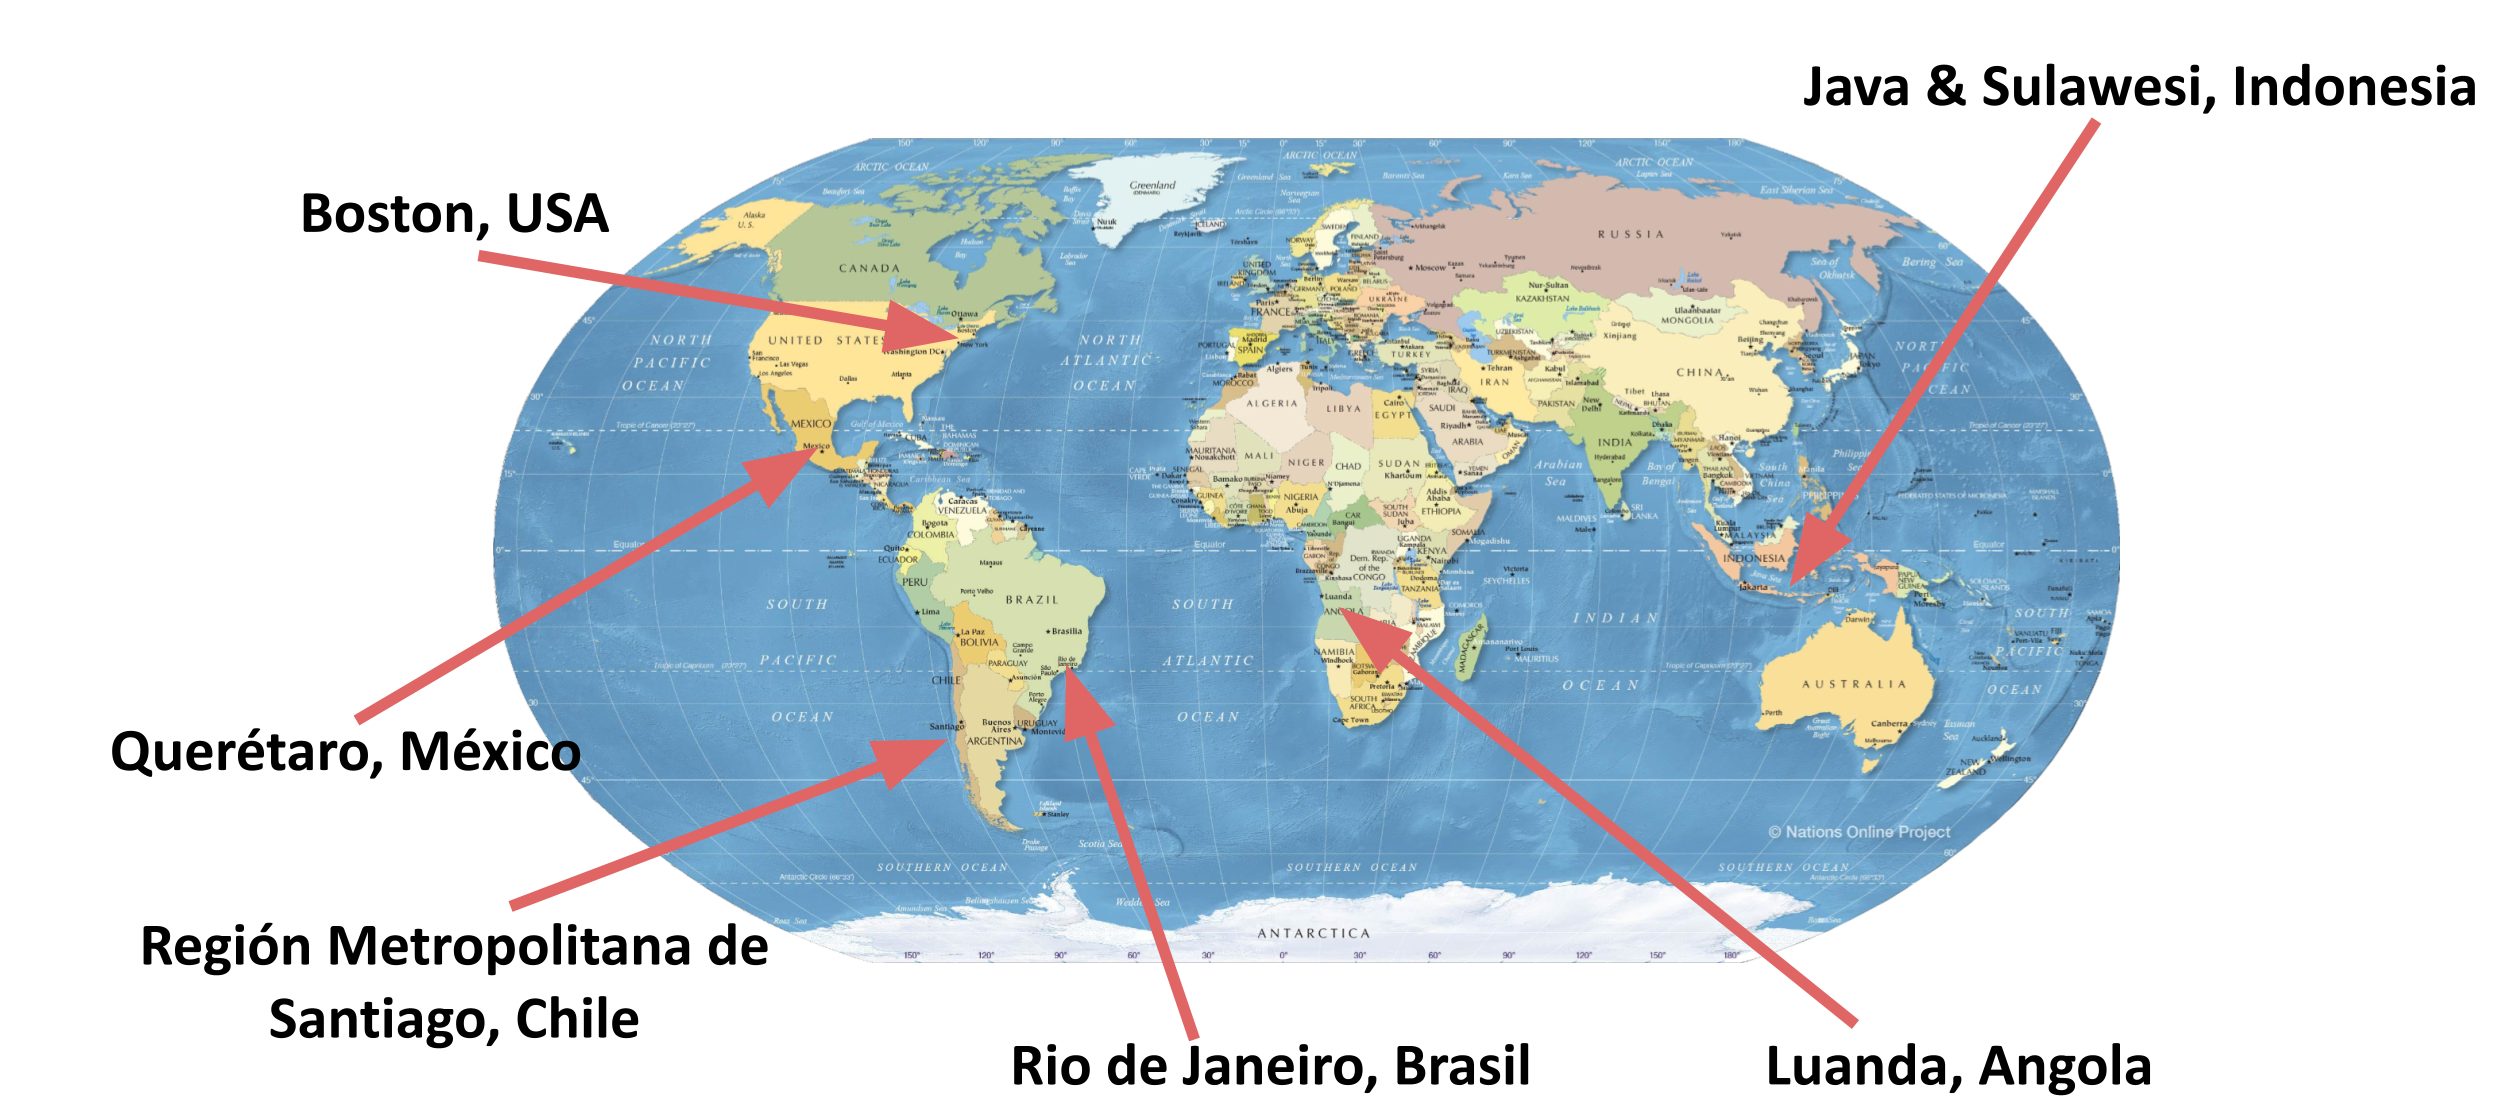
\includegraphics[width=0.9\textwidth]{Figures/chap5/vida_map.png}
	\caption{Metropolitan areas participating in the Vida DSS International Network}
	\label{fig:vida_map}
\end{figure}


Whereas the first case study focuses on simulating the changes in mangrove forest over decades, the focus of Vida is examining hourly to weekly air and water quality data alongside daily coronavirus epidemiological data and weekly quarantine policies. Government officials need actionable data to both address the ongoing public health crisis and to cope with the resultant socioeconomic and environmental consequences. Community members need to understand why their government is making the decisions that it is and understand the risks associated with their own actions. The analysis of System Context will include existing public health infrastructure in these metropolitan areas, how vulnerable they are to epidemics, and how decision-making occurs.  


\subsubsection{\hlc[yellow]{Analyze System Stakeholders}}

The Technical Area Experts on this project included researchers from Harvard Medical School and \ac{nasa} Goddard Space Flight Center. Meanwhile the Local Area Experts (many of whom are technical experts in their own right) included a mix of government officials and academic researchers, most of whom work in the public health and/or in \ac{gis}. The government officials themselves span several different offices, including public health departments, data management authorities, science ministries, and space agencies. The full list of Technical Area Experts and Local Area Experts are shown in Table [**insert table number] The intended Users are those same individuals as well as the various public health agencies / task forces that they are affiliated with.  Participation in the Vida \ac{dss} International Network was directed at two ends: (1) development of the Vida \ac{dss} to conduct analyses and presentations that can inform pandemic response; and (2) sharing more general information and resources among the participants for responding to the pandemic \cite{lombardoDesigningDecisionSupport2020}.

[** insert table listing all experts]]

%Due to the urgent nature of the situation, no formal interviews were conducted at the beginning of the project, unlike the approach taken in Chapter \ref{ch:mangroves}. Instead, a higher tempo of remote meetings were conducted to provide for quicker feedback. This included weekly or biweekly one-to-one meetings (Space Enabled researchers and representatives of one the metropolitan areas) and monthly multilateral meetings (including Technical Area Experts, Local Area Experts, and other guests from all of the metropolitan areas). These meetings allowed for local stakeholders to identify site-specific needs and thereby inform the \ac{dss} architecture; surface, provide, and integrate relevant data products, particularly those generated in-situ by government authorities; participate in the design and implementation of the \ac{dss} prototypes; and evaluate the prototypes.

The Network is constituted by a mix of academic researchers, government officials, and private consultants, chosen for both their field-specific expertise and their familiarity with one or more of these locations of interest.

\subsubsection{\hlc[red]{Understand Desired Outcomes \& Objectives}}

\subsubsection{\hlc[red]{Select System Functions}}

\subsubsection{\hlc[red]{Assign Functions to Forms}}

\subsubsection{\hlc[red]{Monitor and Evaluate Systems}}

\subsection{\hlc[red]{SAF Results}} \label{sec:vida-saf-result}

\subsubsection{\hlc[red]{System Context}}


The second was a recognition that the impacts of and responses to the pandemic can be characterized as a complex system, thus warrenting the kind of multidisciplinary, model-based approach of which \ac{evdt} is an example \cite{deweckHandlingCOVID192020}.

\begin{figure}[H] 
\centering
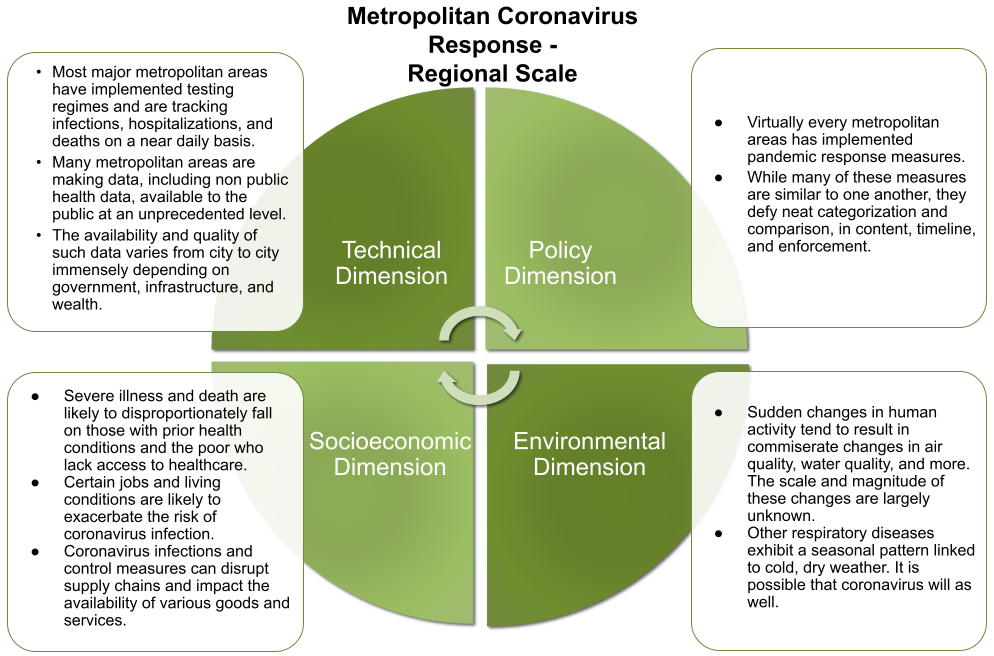
\includegraphics[width=0.8\textwidth]{Figures/chap5/dimensions_vida.png}
\caption[Vida System Context Dimensions]{Vida System Context Dimensions}
\label{fig:dimensions_vida}
\end{figure}


\subsubsection{\hlc[red]{Analyze System Stakeholders}}

\subsubsection{\hlc[red]{Understand Desired Outcomes \& Objectives}}

\subsubsection{\hlc[red]{Select System Functions}}

\subsubsection{\hlc[red]{Assign Functions to Forms}}

\begin{figure}[H]
	\centering
	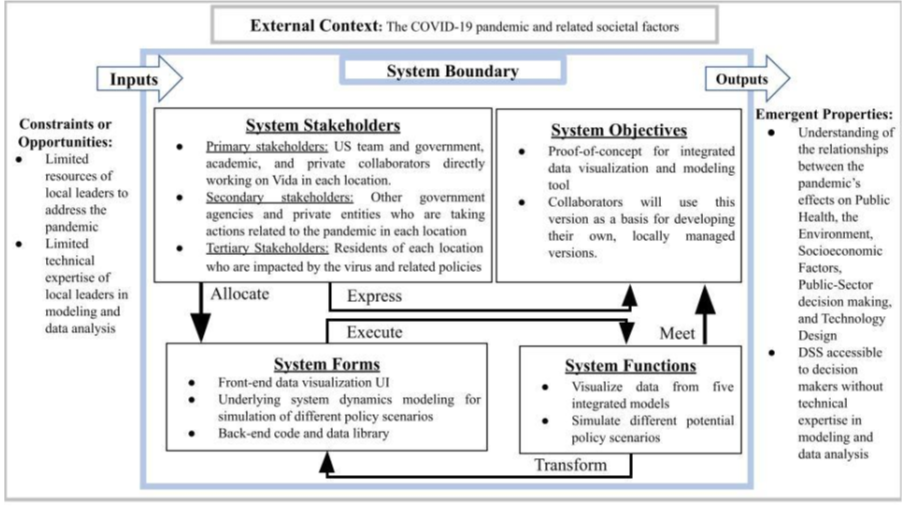
\includegraphics[scale=0.4]{Figures/chap5/architecture.png}
	\caption{The high-level functional systems architecture of the Vida \ac{dss}.}
	\label{fig:architecture}
\end{figure}

\subsubsection{\hlc[red]{Monitor and Evaluate Systems}}

\section{\hlc[cyan]{EVDT Application}} \label{sec:vida-evdt}

he following subsections walk through the components of the system from an \acf{evdt} perspective, detailing what models were used and the results of those models. Before proceeding though, it is worth stating what exactly each of the four components of \ac{evdt} mean for this system. The onset of the COVID-19 pandemic was an immensely significant event around the world. Thus, while it would have been possible to consider public health as a component of the Vulnerability model, in order to properly center and prioritize the public health aspects of the pandemic, a dedicated Public Health Model was added to the default \ac{evdt} arrangement, as shown in Figure \ref{fig:vida_flow}. Returning to the four questions from Section \ref{sec:evdt-questions} (plus one additional one), we ask the following:

\begin{enumerate}[itemsep=0pt,parsep=0pt]
	\item \textbf{What is happening in in public health?} How is the COVID-19 pandemic spreading through the community? What portion of the infected are being hospitalized or dying? What factors impact transmission?
	\item \textbf{What is happening in the natural environment?} How are air quality, water quality, and nightlights being altered by pandemic-related changes in human activity? What role does weather, smog, and other aspects of the environment have on COVID-19 transmission and symptoms?
	\item \textbf{How will humans be impacted by what is happening in the natural environment and in public health?} Who is at most risk of falling ill or suffering from severe symptoms? How are pandemic response policies affecting different populations? Do pandemic-related changes in air quality have a noticeable impact on the residents of these metropolitan areas? How are different industries impacted by such sudden changes in both supply and demand?
	\item \textbf{What decisions are humans making in response to environmental factors and why?} What are the different forms of pandemic response measures being taken by governments, both local and national? How are individual people altering their patterns of work, shopping, and recreation?  
	\item \textbf{What technology system can be designed to provide high quality information that supports human decision making?} What testing regime is needed to effectively reduce the spread of the virus and resultant deaths? What other data sources are useful for informing decision-making?
\end{enumerate}

We can now discuss what approaches were taken for each of these components before presenting their outcomes.

\begin{figure}[H]
	\centering
	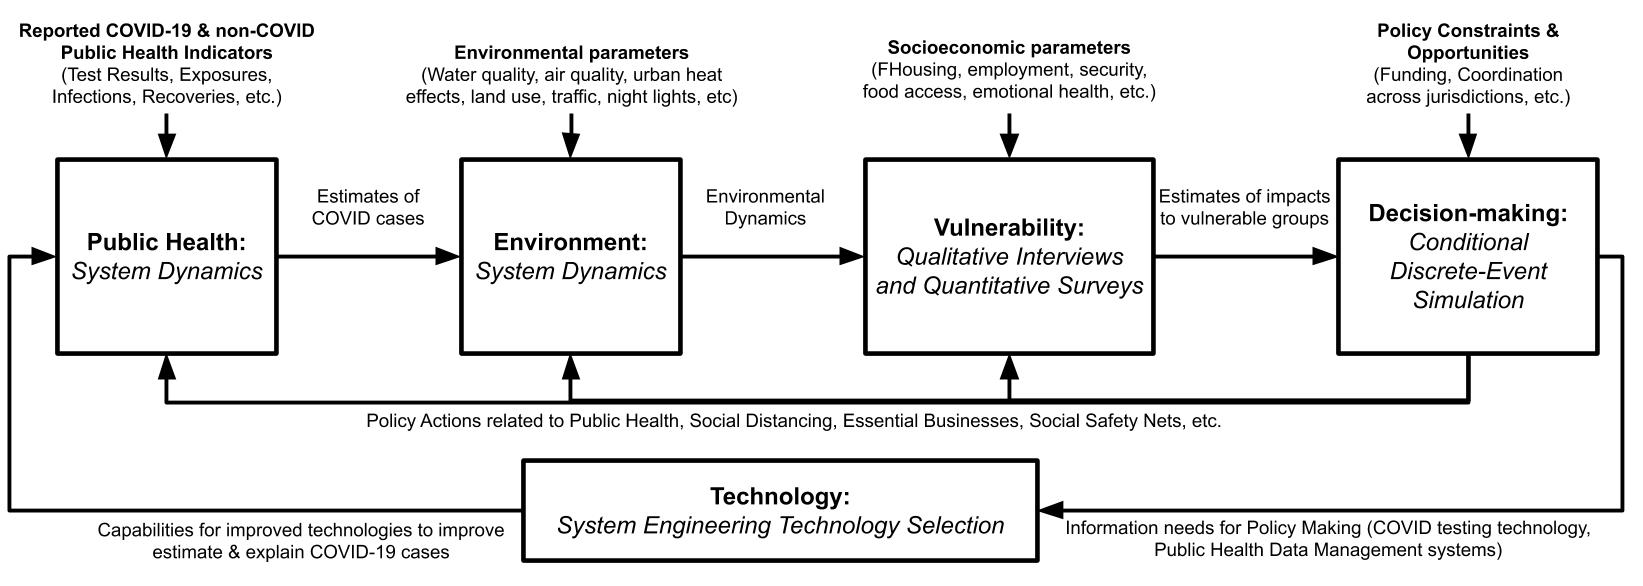
\includegraphics[scale=0.25]{Figures/chap5/Vida_Flowchart_v2.jpg}
	\caption[The Vida Variant of the EVDT Model]{The Vida variant of the EVDT model, designed to support decision making by governments during COVID-19}
	\label{fig:vida_flow}
\end{figure}

\subsection{\hlc[cyan]{EVDT Methodology}} \label{sec:vida-evdt-method}


\subsubsection{\hlc[cyan]{Environment}} \label{sec:vida-evdt-e-method}

Unlike the previous case study, which focused on a particular aspect of the environment (mangroves) that had an established literature, the onset of the COVID-19 pandemic resulted in many disparate impacts on the environment in quick succession. As discussed earlier, it also was not immediately clear what topics were the highest priority to stakeholders. As a result, many areas were explored and only some pursued in detail.

Urban nighttime lighting patterns changed and (generally) dimmed \cite{elvidgeDimmingLightsChina2020}. Air quality noticeably improved as traffic patterns changed and work-related emissions declined \cite{isaifanDramaticImpactCoronavirus2020}. In many places, water quality noticeable improved and noise diminished \cite{aroraCoronavirusLockdownHelped2020}. We pursued these using both remote sensing data (Landsat and Sentinel for air and water quality estimations, VIIRS for nighttime lighting, Planet and Sentinel SAR for traffic pattern changes) and in-situ sensors (such as the Rio de Janeiro MonitorAr program's air quality sensors).

For nightlights, the VIIRS VNP46A2 dataset was used \cite{romanNASABlackMarble2018}. This dataset contains daily panchromatic (visible and NIR) imagery at at a resolution of 15 arc-seconds (approximately 450m for the locations of interest) that has been corrected for atmospheric interference and moonlight variation. It is thus well suited for examining artificial lights, such as those generated by cities. We process it by masking out clouds and water (thereby eliminating transient lights from ships) using the supplied quality flag, then taking weekly median values to reduce intraweek variation, before calculating the relative anomaly compared to the 2019 median value for each pixel, thereby standardizing comparisons across time and space. We can then compare specific pre-and-post pandemic time periods to identify changes. Further normalization can be performed by identifying any long term trend from Jan 1st, 2019 to March 1st, 2020 (the approximate start of the pandemic) and subtracting this extrapolated trend from the post-pandemic data. This methodology is summarized below in Figure \ref{fig:nightlights_method}.

\begin{figure}[h]
\centering
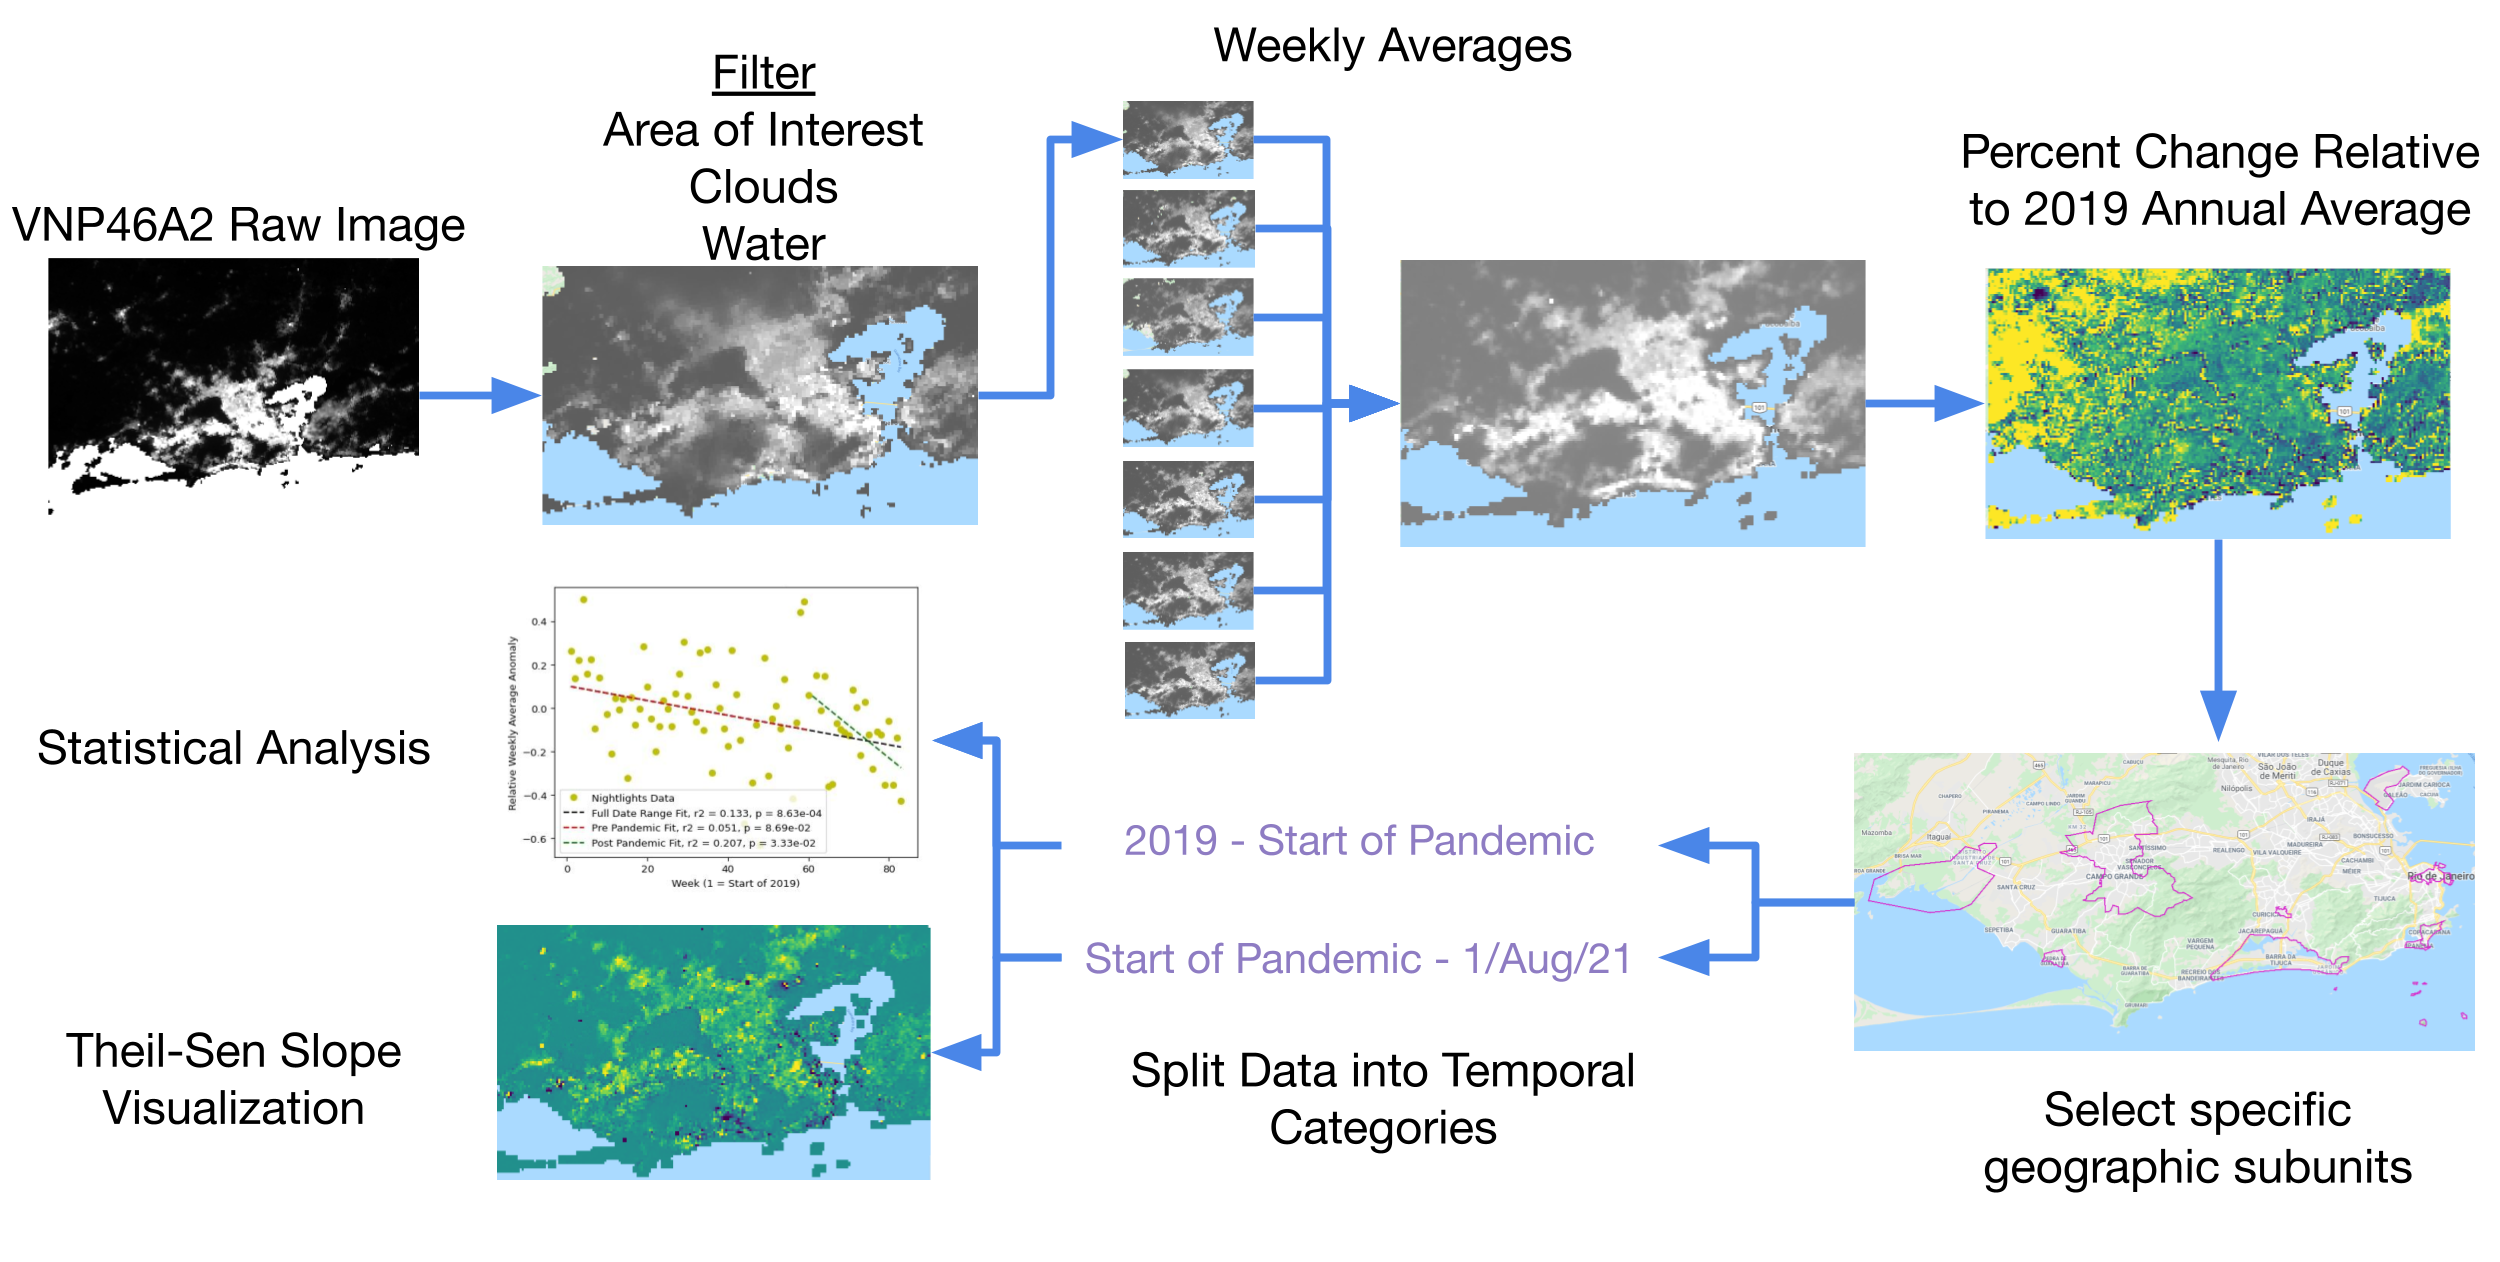
\includegraphics[width=0.9\textwidth]{Figures/chap5/nightlights_method.png}
\caption[Nightlights Processing Methodology]{Method for processing and analyzing nightlight data}
\label{fig:nightlights_method}
\end{figure}

For air quality, data from Rio de Janeiro MonitorAr air monitoring stations was used. In-situ sensors take hourly measurements to monitor a range of air quality parameters (e.g O3, CO, SO2, PM10, etc.) in 8 different barrios, or neighborhoods, of Rio de Jeneiro. The dataset is provided publicly and freely through Rio de Janeiro's Data.Rio website \cite{institutopereirapassosDataRio2017}. For the purposes of this study, we focused on changes in the measured PM10 pre-and-post pandemic. We process the data for each barrio by first calculating weekly averages to reduce intraweek variation, as we would expect there to be a difference in air emissions throughout the week (for instance, weekends versus weekdays). Then the data was fit using a least-squares estimate to a sinusoidal wave with an annual period. This sinusoidal curve is the average seasonal variation in PM10 for that barrio, and it is subsequently subtracted out from the data. A best-fit line is then calculated for this seasonally-corrected data. The best-fit line is long-term (multi-year) trend in PM10 measurements, and it is also subtracted out. At this point, the data is corrected for intraweek, seasonal, and annual trends, and we can then construct normalized histograms and compare the pre-and-post pandemic distributions to identify changes and trends. Similar analyses have been conducted using Chile's Sistema de Información Nacional de Calidad del Aire \cite{ministeriodecienciatecnologiaconocimientoeinnovacionDatosCOVID192021} for the Santiago area.

Some experimentation was performed in assessing changes in air quality and traffic patterns in Rio de Janerio using \ac{eo} imagery. Further meetings with stakeholders suggested that this was of limited usefulness, particularly in the other locations. This, coupled with a lack of accessible validation data, resulted in us abandoning such efforts.

\subsubsection{\hlc[cyan]{Public Health}}

The most notable variation that Vida has compared to previous \ac{evdt} applications is the addition of a dedicated Public Health Model. While the specific data collection definitions, coverage, and update cycles vary, each of the participant locations collected and published coronavirus-related epidemiological data on a regular basis, including newly identified infections, deaths, hospitalizations, etc. Vida ingests this data and uses it both to display historical trends alongside the other components and to conduct simulations of potential future behavior, with an emphasis on future trajectories of infections and hospitalizations. The Public Health component is based on a \ac{sir} system dynamics model. \ac{sir} is a compartmental epidemiological model and one of the most commonly used variants, due to its relative simplicity and flexibility. System dynamics is a modeling approach commonly used in both 'pure' epidemiological contexts \cite{homerSystemDynamicsModeling2006} and in broader public health policy contexts \cite{deutschCommunitybasedSystemDynamics2020}. Figure \ref{fig:vida_sd} shows a diagram depicting the layout of the Vida Public Health Model. In addition to the three traditional \ac{sir} components, it has two other health compartments: Hospitalizations and Deaths. These reflect some of the primary decision points and metrics of performance that policymakers are using. In most of our application contexts, population counts for each of these compartments is readily available on a daily or weekly basis. 

In the top left and bottom left of the diagram, the initial inclusions of Environment and Vulnerability components are shown. These are obviously cursory and highly assumptive. Air pollutants, for example, are not merely a function of closure policy. In most locations that we have examined, and in research conducted by others \cite{isaifanDramaticImpactCoronavirus2020}, initial coronavirus-related closures resulted in a sudden drop of emissions (further discussion on this in the Section \ref{sec:vida-evdt-result}). Furthermore, there is some evidence that weather and air pollution have a modest impact on COVID-19 transmission \cite{xuModestImpactWeather2020}, leading to the inclusion of such an element in the top left of the diagram.

This model is non-spatial, though in some locations of interest with distinct geographies (such as the Indonesian islands of Java and Sulawesi), multiple independent instances of the model are generated.

\begin{figure}[h]
	\centering
	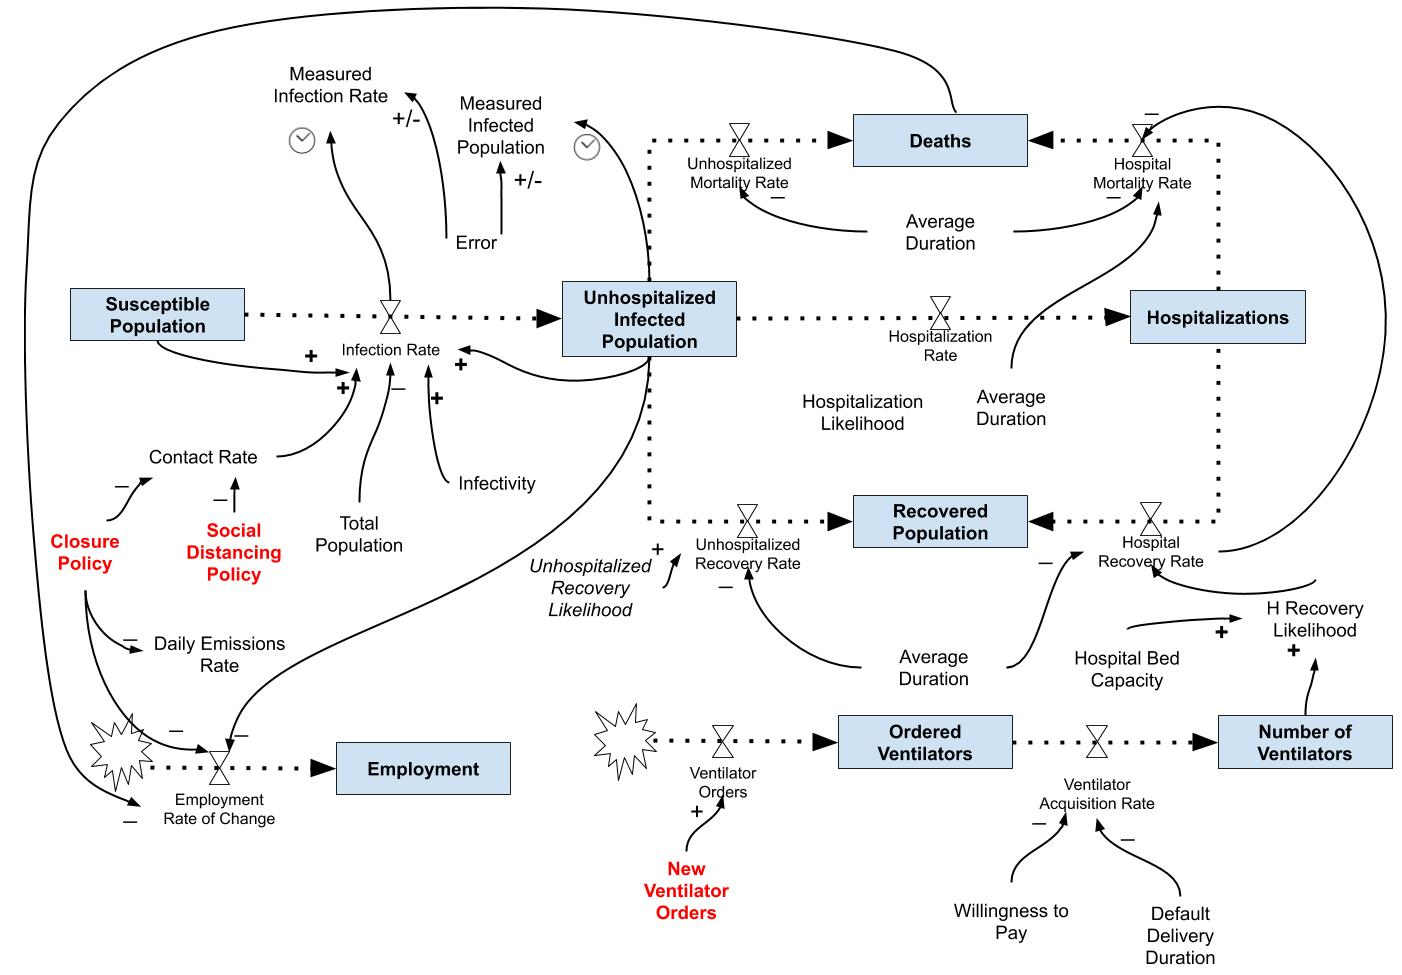
\includegraphics[scale=0.25]{Figures/chap5/SD_diagram.jpg}
	\caption[Current version of the Vida SIR system dynamics model]{Current version of the Vida \ac{sir} system dynamics model}
	\label{fig:vida_sd}
\end{figure}


\subsubsection{\hlc[yellow]{Vulnerability}}

Traditional, government-collected socioeconomic impact data largely does not exist at the fine temporal resolution required for coronavirus-related assessment, so we had to develop the Invisible Variables Initiative (not discussed at length in this thesis) to work with our collaborators to develop surveys and interview procedures to elicit needed information. This initiative is led by Dr. Katlyn Turner and funded by the Natural Hazards Center at the University of Colorado, Boulder. As the pandemic progressed, however, some more traditional metrics, such as unemployment data, that show responses to the crisis began to be released.

Another aspect of societal impact and vulnerability that Vida monitors is mobility. This includes movement as demonstrated by telecommunications activity, automobile traffic, air traffic, and ship activity, the last of these primarily of relevance to the Luanda stakeholders. Telecommunications activity is being made in numerous jurisdictions either directly by private companies \cite{googleCOVID19CommunityMobility} or via government data repositories \cite{ministeriodecienciatecnologiaconocimientoeinnovacionDatosCOVID192021} and integrated into Vida. Data on air traffic is commonly collected and published by local government authorities. Data on ship activity can be generated through the use of Sentinel radar imagery by masking out land and permanent structures, then looking for transient bright spots on navigable bodies of water, particularly around major ports. This process can be seen in Figure \ref{fig:ships}. The period of 2018 through the start of the pandemic was used to establish a baseline of ship presence. This was then compared with activity after the onset of the pandemic to identify changes. 

\begin{figure}[h]
	\centering
	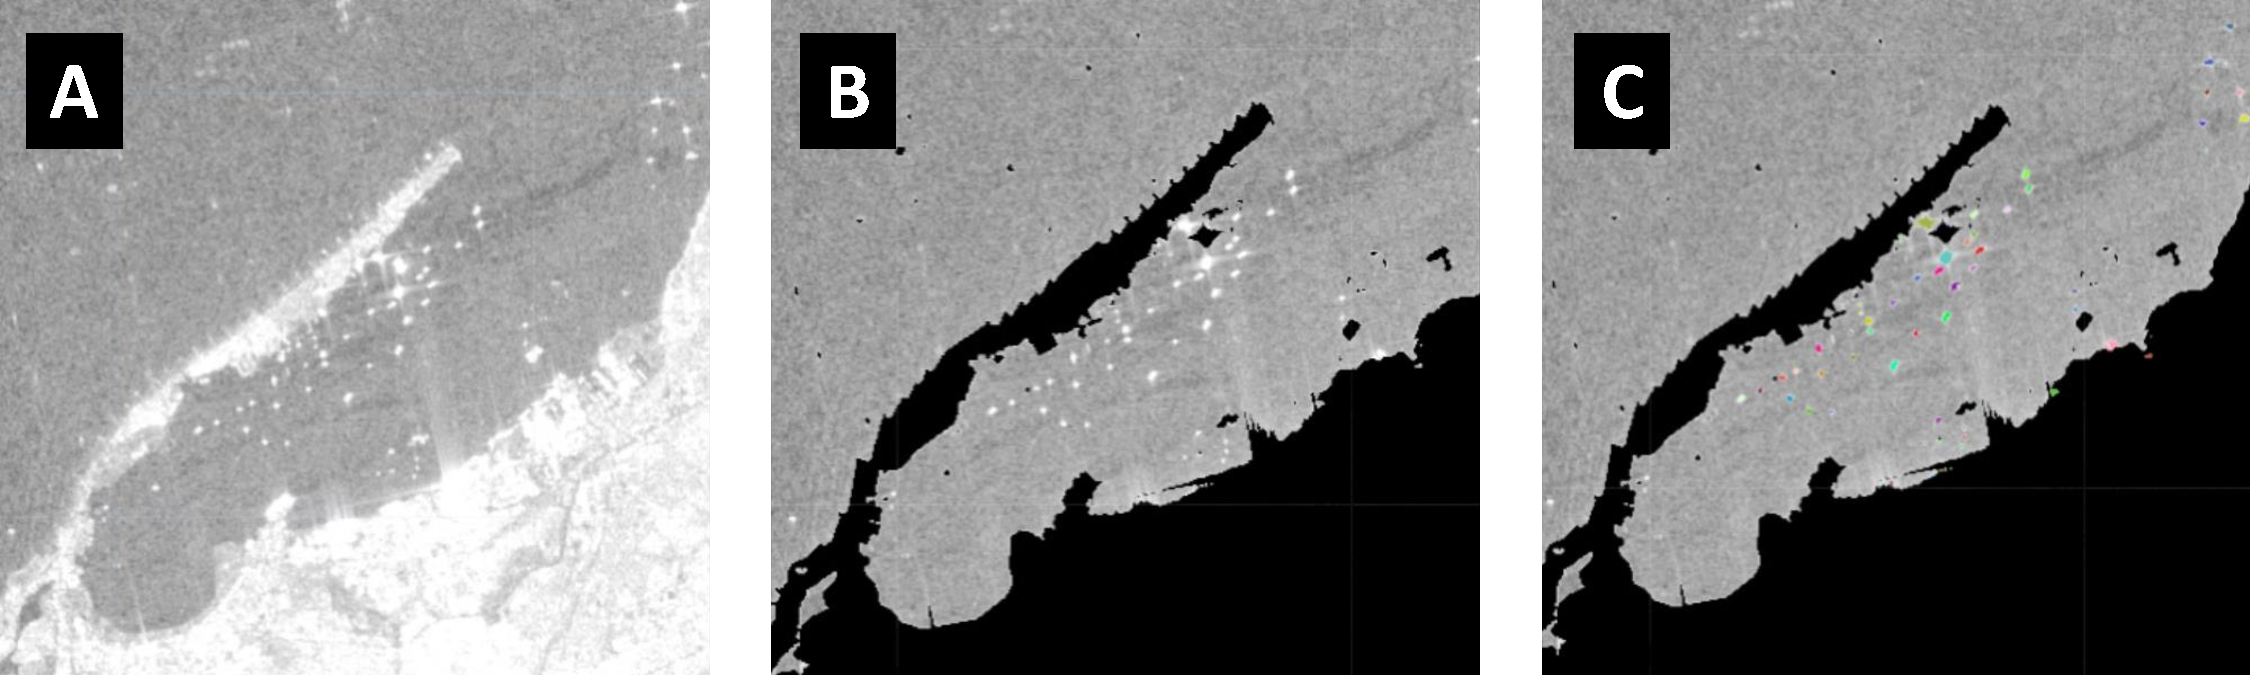
\includegraphics[scale=0.35]{Figures/chap5/ships.pdf}
	\caption[Ships identification process]{Ships identification process. A: Sentinel-1 SAR imagery of the Luanda area. B: Masking out land and permanent structures. C: Identifying individual ships. Figure created by Amanda Payton.}
	\label{fig:ships}
\end{figure}

[** add explanation of the mobility methodology]


\subsubsection{\hlc[cyan]{Decision-making}}

Obviously the primary decision axis is containing the spread of coronavirus and properly treating those who are infected. In practice this tends to express itself as various forms of public area and business closures and restrictions, individual social distancing requirements (such as mask wearing), and medical equipment acquisition and allocation. In Rio de Janeiro, for example, many of these policies have been grouped together into a six phase Resumption Plan that has clear indicator-based conditions for when to advance to the next phase \cite{iplanrioIndicadoresPlanoRetomada2020}, which facilitates visualization and simulation in Vida. Most of the locations of interest have similar qualitative, ordinal policy categories, with varying numbers of steps or details. 

We spent some effort at developing a consistent process for transforming such policies from qualitative ordinal categories into quantitative scores, building upon such projects as the CoronaNet Research Project \cite{CoronaNetResearchProject}. This was done both to enable consistent visualizations where various quantitative metrics (active coronavirus cases, air quality, mobility indices, etc.) can be directly compared to policy actions over time (e.g. in Fig \ref{fig:mob}). It also would enable some level of comparison across locations of interest in order to help draw causal relationships and identify the impacts, both positive and negative, of certain policies. Our approach to this was to break policies into different categories (e.g. social distancing / masking requirements, business closures or capacity limitations, travel restrictions, etc.) and define specific ranks within such category (e.g. no outdoor events with greater than 15 people vs no outdoor events with greater than 50 people). The local teams for each location of interest were involved in both the definition of these ranks and the categorization of local policies into them. Ultimately the Vida project concluded prior to this quantification process being completed.  

\subsubsection{\hlc[yellow]{Technology}}

Various forms of sensing technology are relevant during a viral epidemic. While our team has remained primarily focused on satellite-based earth observation technology and in-situ environmental sensors, another key form of relevant sensing technology is coronavirus testing (both the technology of the individual tests and the social technology that is the regional testing regime). Rates of testing can be integrated into the public health model through its influence on the difference (or lack thereof) and delay between the estimated number of active infections and the measured infections.

\subsection{\hlc[red]{EVDT Results}} \label{sec:vida-evdt-result}

\subsubsection{\hlc[yellow]{Environment}} \label{sec:vida-evdt-e-result}

We ran two-samples t-tests and Anderson Darling tests on the normalized histograms of the pre-and-post pandemic variation-corrected PM10 data, assuming that the pre-pandemic distribution was approximately normally distributed. These tests determine if the pre-pandemic and post-pandemic PM10 measurements are actually different. In particular, as seen in Figure \ref{fig:pm}, we found that tourist areas had a significant decrease in measured PM10 post-pandemic, while some rural or residential areas had slight decreases. We found a significant increase in PM10 measurements post-pandemic in the downtown/business district, with some smaller increases in mixed use/residential and recreational areas. 

\begin{figure}[h]
\centering
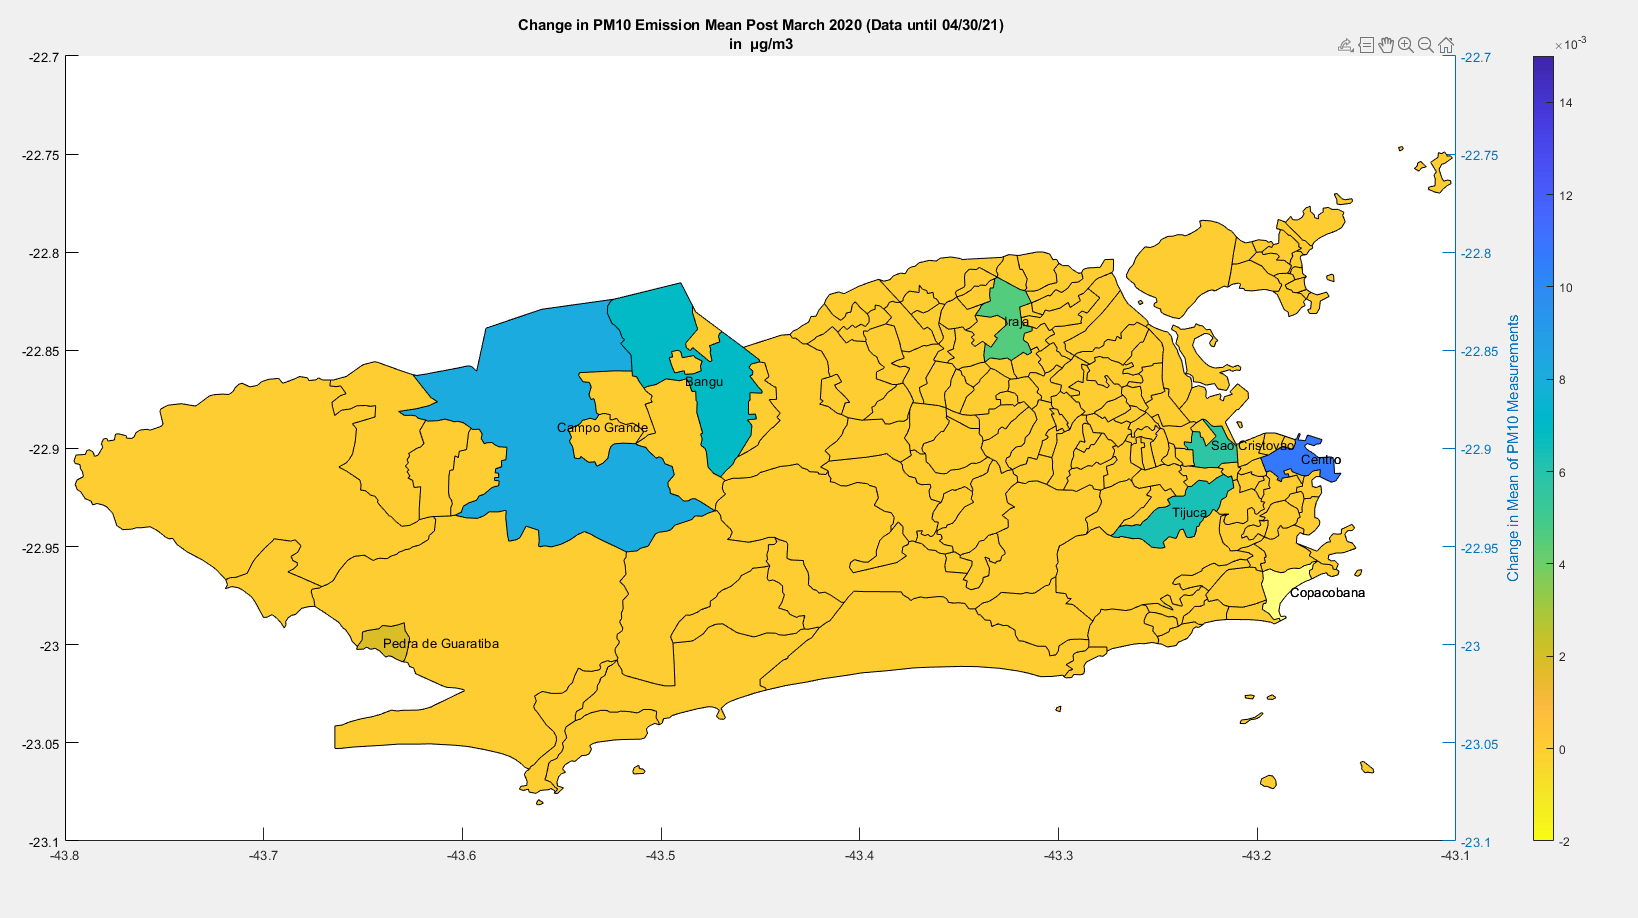
\includegraphics[width=0.9\textwidth]{Figures/chap5/pm10.png}
\caption[Changes in PM10 in Rio de Janeiro]{Changes in PM10 levels in several bairros of Rio de Janeiro during the first two months of the pandemic, normalized for intraweek, seasonal, and annual trends.}
\label{fig:pm}
\end{figure}

Similarly to other researchers, we detected significant changes in nightlights due to the onset of COVID-19 and later policy changes \cite{elvidgeDimmingLightsChina2020, xbsdScipy2021Predicting2021}. In particular, areas associated with air travel and tourism experienced significant decreases in nightlights and associated human activity (areas in purple along the eastern and southern edges of Rio de Janeiro in Figure \ref{fig:nlts}). Downtown and commercial areas experienced a similar, though less dramatic decrease. Primarily residential areas (the yellow, east-west arc across the middle of Figure \ref{fig:nlts}), meanwhile, significantly brightened. These trends are apparent both for relative percentage change across these areas and when the changes are normalized for long term trends. Graphs showing such changes for airports and specific tourist-centric areas in Rio de Janeiro, Brazil and Bali, Indonesia can be seen in Figure \ref{fig:nlg} of the Appendix. The results of basic statistical analysis, particularly t-tests to determine if pre-pandemic and post-pandemic brightness are actually different, for various bairros and areas of Rio de Janeiro can be seen in Figure \ref{fig:nstats}.

\begin{figure}[h]
\centering
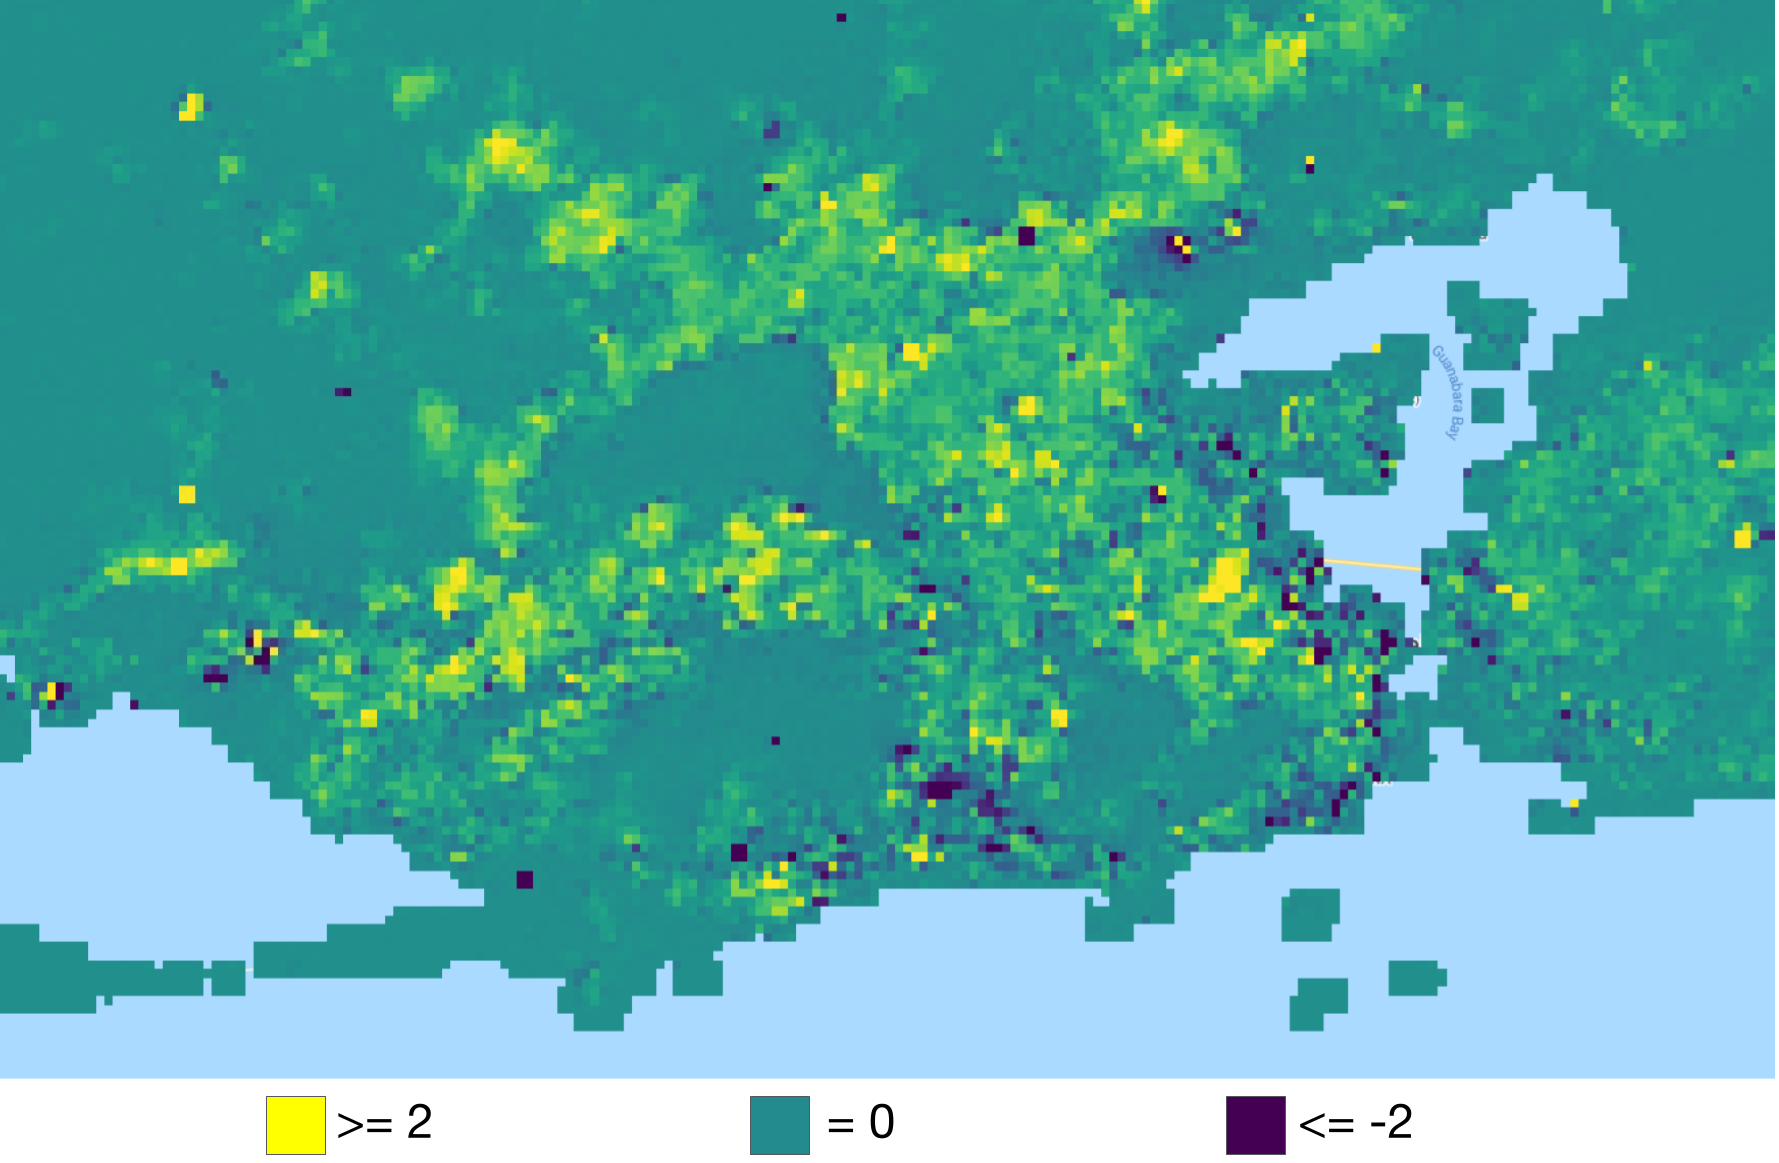
\includegraphics[width=0.9\textwidth]{Figures/chap5/Nightlights_TS.png}
\caption[Changes in nightlights in Rio de Janeiro]{Theil-Sen trend estimator for normalized changes in nightlights in Rio de Janeiro during the initial phases of the pandemic (March 1st to August 30th, 2020).}
\label{fig:nlts}
\end{figure}

\begin{figure}[H] 
\centering
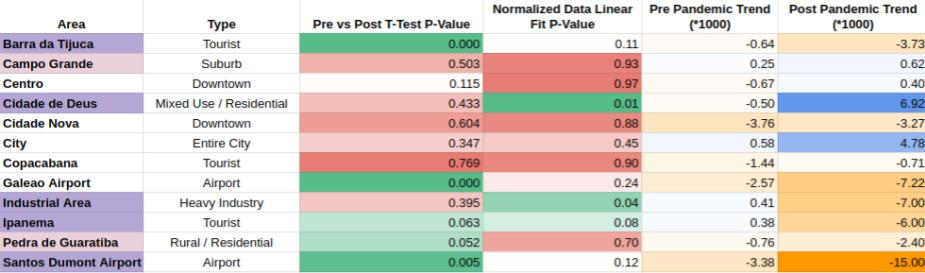
\includegraphics[width=0.9\textwidth]{Figures/chap5/RioNightStats.jpg}
\caption[Nightlight Statistics for Rio de Janeiro]{Statistics for nightlight trends in several bairros (neighborhoods) and areas of Rio de Janeiro. Greens indicate stronger statistical significance, red less. Yellows indicate negative trends, blue positive.}
\label{fig:nstats}
\end{figure}


\newpage

\begin{figure}[H] 
\centering
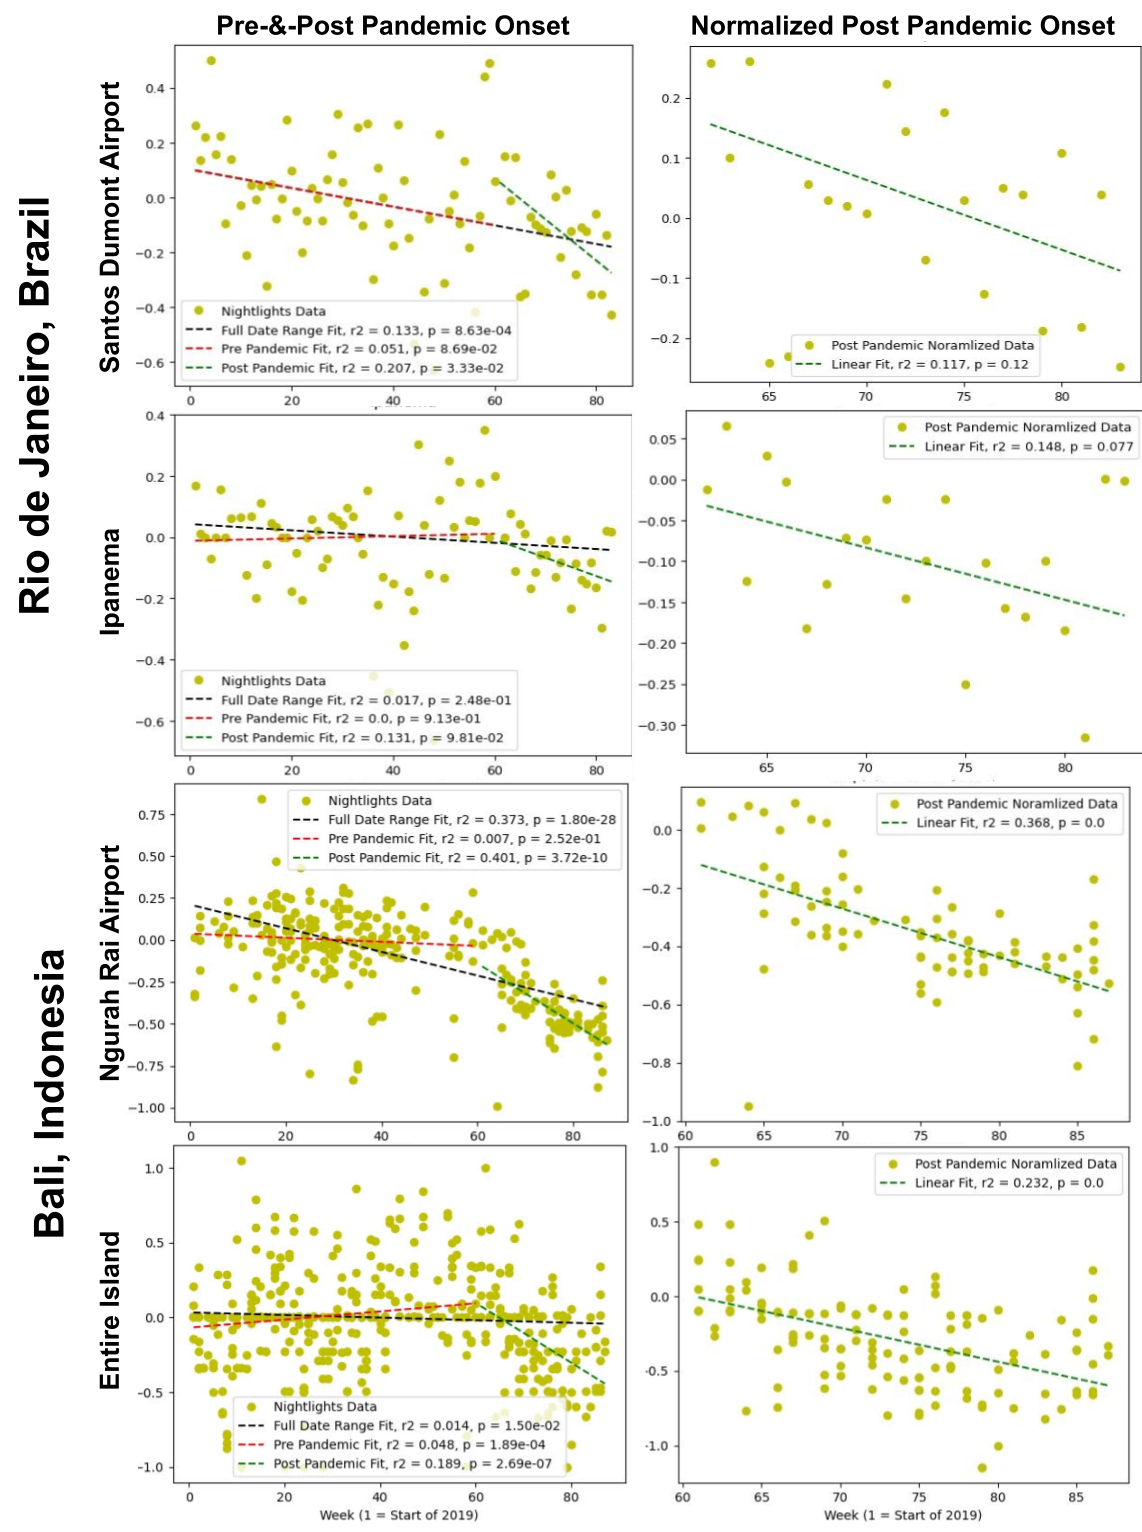
\includegraphics[width=0.85\textwidth]{Figures/chap5/Nightlights_Graphs.png}
\caption[Nightlight Trends for Rio de Janeiro and Bali]{Pre-and-post pandemic nightlight trends for Rio de Janeiro and Bali, showing both airports and tourist-centric areas.}
\label{fig:nlg}
\end{figure}



\subsubsection{\hlc[yellow]{Public Health}}

In addition to presenting historical data, the desktop version of the \ac{dss} can also conduct public health simulations, using the system dynamics \ac{sir} model presented earlier. This simulations can either be run manually, with the user selecting specific policies at each week using the controls in the bottom left, or automatically for specified time periods, according to certain pre-coded decision rules (listed in the bottom right) based on the official policies of the location of interest.

This model is currently being calibrated using historical data, expanded as new dynamics become evident, and examined by public health experts. Various potential improvements are evident, including combining the \ac{sir} system dynamics model with an agent-based model to help address some of the deficiencies of the system dynamics approach \cite{ahmedVarianceSystemDynamics2012}, such as the lack of a spatial component.

\subsubsection{\hlc[yellow]{Vulnerability}}

Telecommunications-based measurements of Vida have also provided insightful for decision-makers. Figure \ref{fig:mob} compares mobility with active coronavirus cases and policy status in Santiago, Chile and Rio de Janeiro, Brazil. Some variations are unsurprising: a upward spike during Chile's constitutional referendum, downward spikes for the winter holidays. Others are more relevant for policy-making. Specifically, once the number of active cases declines, mobility increases even if policies remain restrictive.

\begin{figure}[h]
\centering
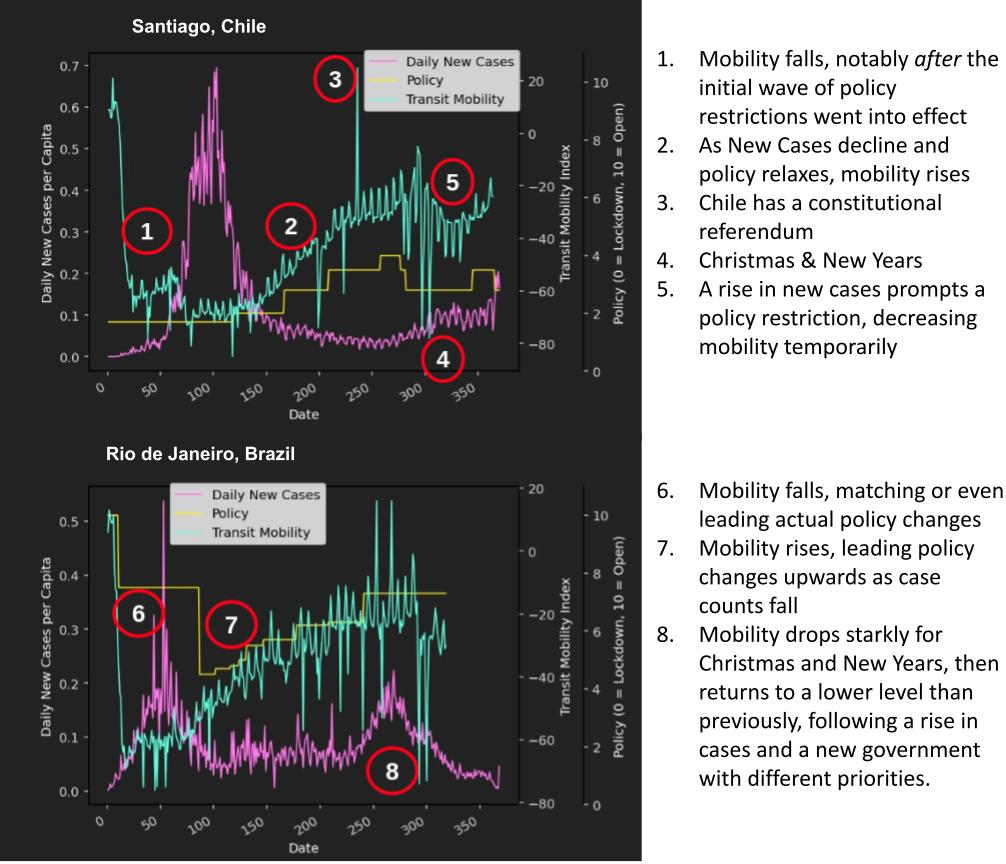
\includegraphics[width=0.9\textwidth]{Figures/chap5/Mobility-Graphs.jpg}
\caption[Mobility, coronavirus cases, and policy changes in Rio de Janeiro]{Comparisons of coronavirus cases, policy changes, and mobility for Santiago and Rio de Janeiro. Day 0 is set at the first confirmed COVID-19 case in that location (04/Mar/20 for Santiago, 07/Mar/20 for Rio de Janeiro).}
\label{fig:mob}
\end{figure}

Initial results regarding ship tracking in the harbor of Luanda, Angola suggest that there may be a visible change in ship number and location related to the pandemic. Compared to the preceding two years, the monthly average number of ships within the Bay increased slightly after the onset of the pandemic and continued to remain higher throughout the year. In the offshore area outside of the bay, the average monthly number of ships was lower than in the two years preceding the pandemic. As the number of COVID-19 cases in the country climbed, the number of ships within the bay further increased, while the number of ships in the offshore area decreased (as shown in Figure \ref{fig:shipst}). The extended docking within the harbor could reflect a reduction in ships conducting trade or delays in the process of loading and unloading ships due to COVID-19.  Further investigation is needed into the accuracy and statistical significance of these results in order to draw conclusions. However, at this early stage of analysis it appears that detecting changes in economic proxies such as ship movement using satellite imagery is possible and we plan to extend our analysis to other regions for comparison.

\begin{figure}[h]
\centering
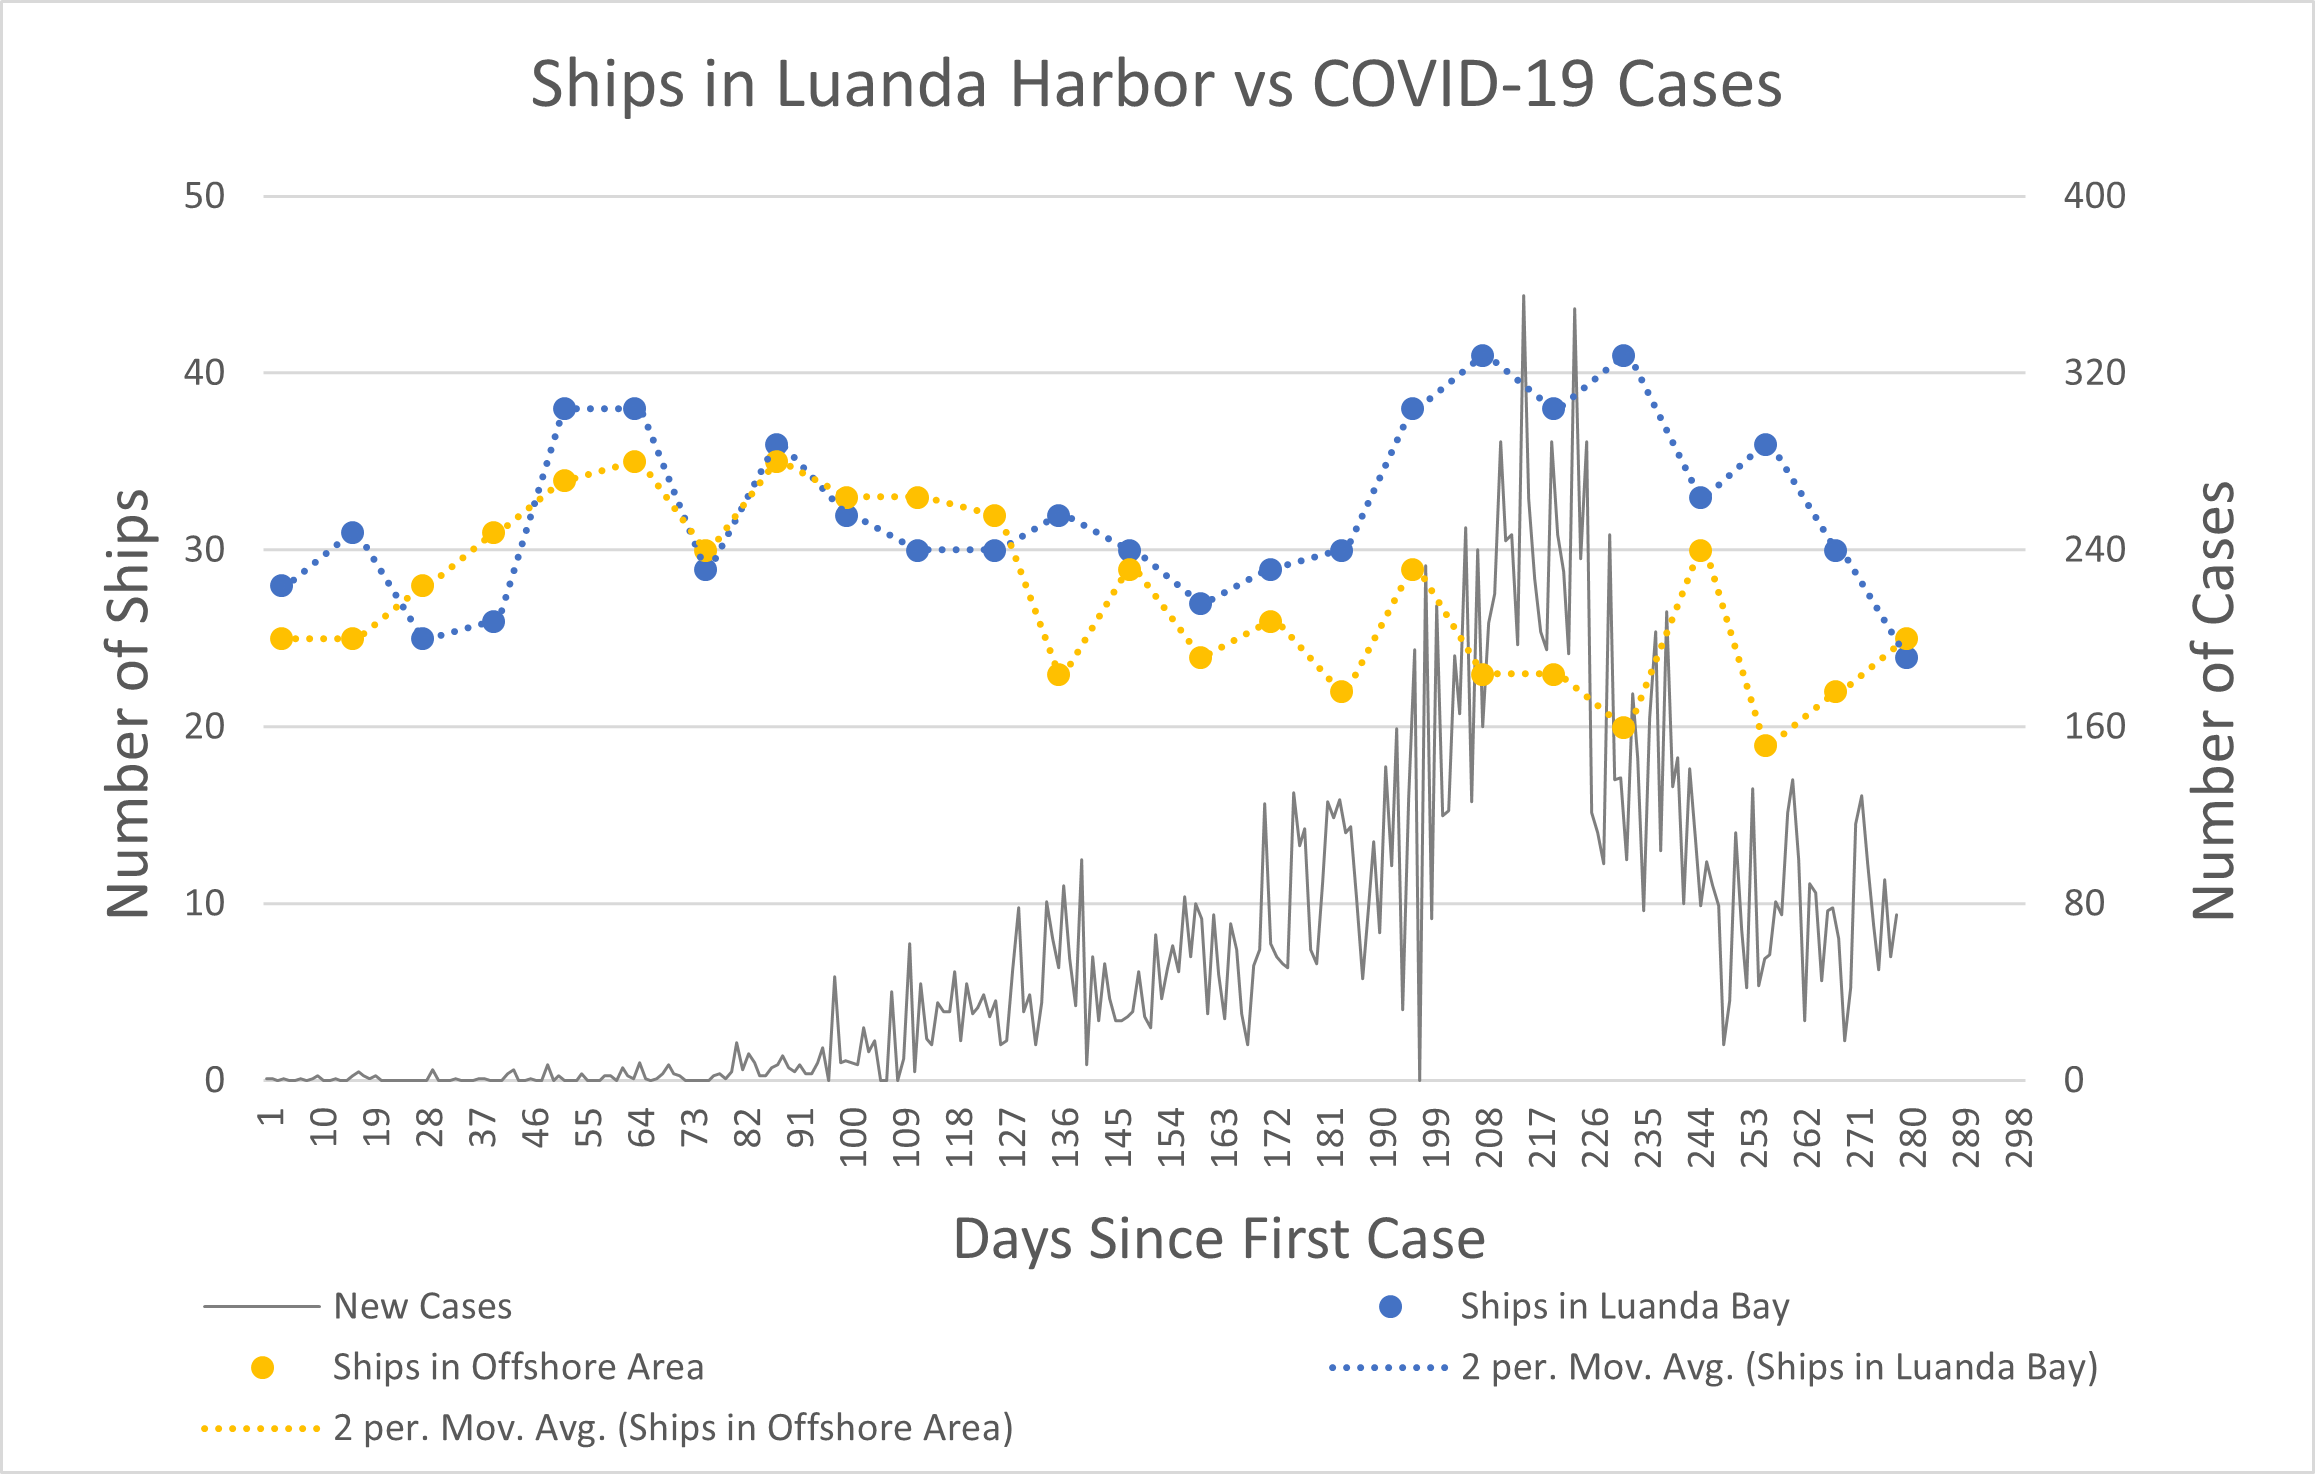
\includegraphics[width=0.9\textwidth]{Figures/chap5/ships_over_time.png}
\caption{Ship presence over time for the Luanda area.}
\label{fig:shipst}
\end{figure}

\subsubsection{\hlc[red]{Decision-Making}}

\subsubsection{\hlc[red]{Technology}}



\section{\hlc[yellow]{Decision Support System}} \label{sec:vida-dss}

At the time of writing, two distinct versions of the Vida \ac{dss} exist, both of which are undergoing active development and should not be viewed as final products. The first, shown in Figure \ref{fig:vidad}, is an open-source, desktop-based version written in Python (the code is available online \cite{reidMITVidaRepository2021}), that can be run on various operating systems (recent versions of Windows, MacOS, and various Linux distros have been tested). 

The user interface can be easily switched between languages (English, Spanish, and Portuguese are currently available, with easy functionality for adding additional languages) and between the locations of interest.

This version can present temporal data, spatial data, and spatiotemporal data. The first of these is done through plots (visible on the left of Figure \ref{fig:vidad}, but the placement of the plots can be reconfigured by the user), with the data visible in the plots controllable through dropdown menus. The other two kinds of data are presented in the kinds of maps shown on the right, which is currently displaying visual imagery of the Rio de Janeiro area overlaid with the most recent PM10 measurements from in-situ monitoring stations. Should either the raster imagery or the vector geographic data be available at multiple points in time, additional slides appear at the bottom of the image to allow the user to select specific dates. Non-spatial data are saved in CSVs, vector spatial data in shapefiles, and raster spatial data in GeoTIFF format.

The goal is not for the authors to continue development of this model indefinitely ourselves, but rather to hand over the model and its associated user interface to local collaborators in each of the application areas, so that they can continue to adjust it to their local circumstances. Other future improvements include more automated ingestion of data from online data repositories, streamlined exporting of visualizations, and making this version accessible online.

The second version of the Vida is online, created in collaboration with Blue Raster and hosted by Esri's ArcGIS Online \cite{bluerasterMITVidaSupportBoston2021}, and has somewhat different functionality. This version, shown in Figure \ref{fig:vidab} (using the Boston areas as an example), focuses on the presentation of historical data and thus lacks simulation capability. It does however have the capability of showing more graphs at the same time, including allowing the user to merge multiple graphs into one for easy comparison, and an overall more streamlined interface.

The remaining portions of the Results section will focus on several specific insights and analysis that have arisen out of the Vida development and use processes.

\begin{figure}[h]
\centering
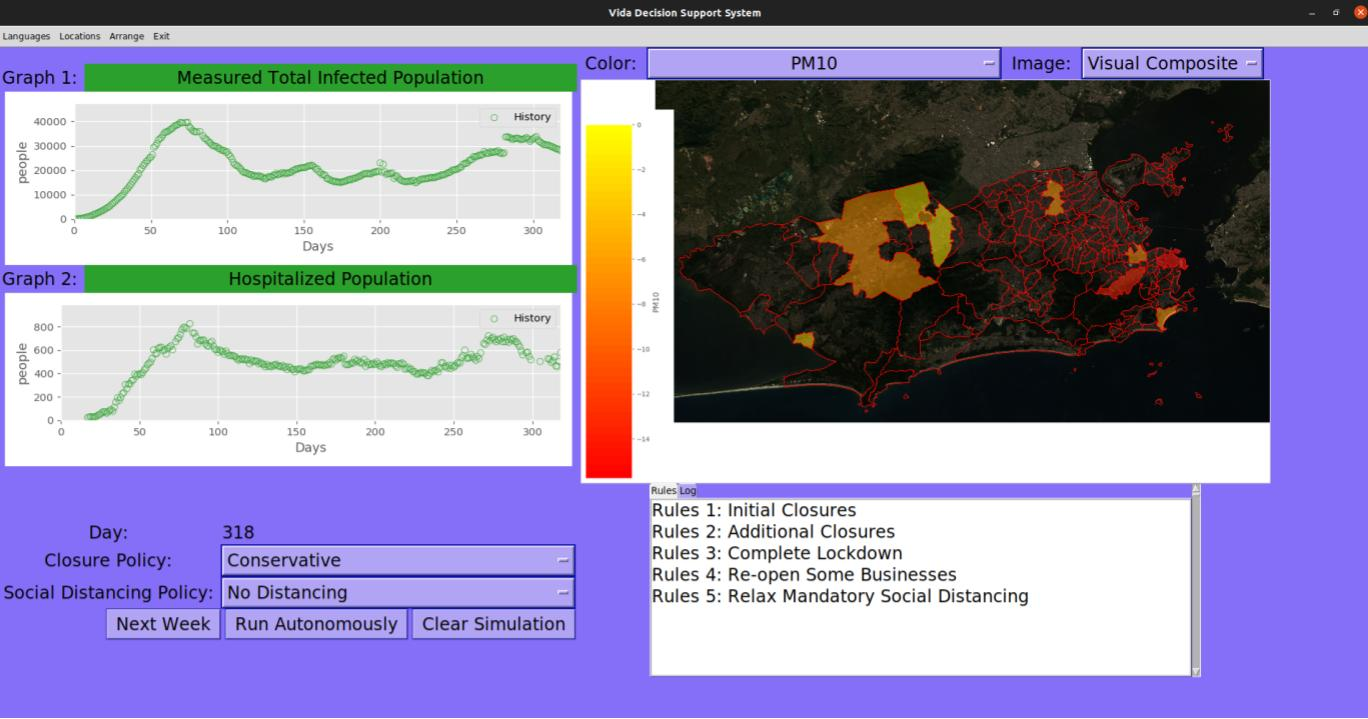
\includegraphics[width=0.85\textwidth]{Figures/chap5/VidaDesktopScreenshot.jpg}
\caption{Prototype of the desktop version of the Vida user interface for Rio de Janeiro.}
\label{fig:vidad}
\end{figure}

\begin{figure}[h]
\centering
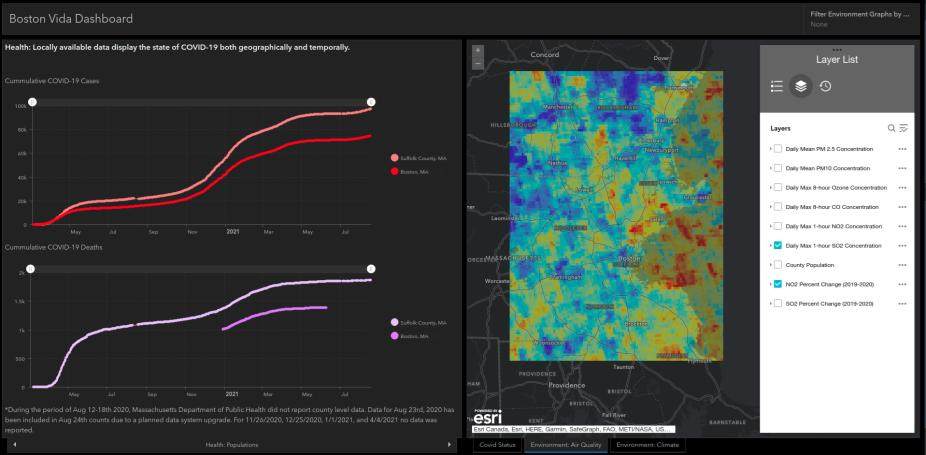
\includegraphics[width=0.85\textwidth]{Figures/chap5/VidaBlueScreenshot.jpg}
\caption{Prototype of the online version of the Vida user interface for Boston.}
\label{fig:vidab}
\end{figure}

\section{\hlc[red]{Collaborative Development Process}} \label{sec:vida-collab}

The second objective of the Network is primarily accomplished through monthly, full Network meetings, at which participants present and discuss useful lessons and tactics for addressing coronavirus response, including topics not directly related to Vida. Examples of such topics are how to implement wastewater viral testing and how to integrate the data generated into decision-making, how to approach health surveillance in elderly care facilities, and how to identify high vulnerability neighborhoods. These discussions promote innovation and enable cross-location learning that may not otherwise occur.

These activities are conducted through weekly or biweekly meetings between the Boston-based research team and individual site representatives and through online collaboration via the local collaborators own online data repositories (e.g. Rio de Janeiro's Data.Rio \cite{institutopereirapassosDataRio2017} or Chile's Datos-COVID19 \cite{ministeriodecienciatecnologiaconocimientoeinnovacionDatosCOVID192021}), the Vida project's own code repository \cite{reidMITVidaRepository2021}, and through interaction with the browser-based version of the Vida \ac{dss} prototype \cite{bluerasterMITVidaSupportBoston2021}.

\section{\hlc[red]{Discussion}} \label{sec:vida-discuss}

Moving forward, work is ongoing to improve the Vida \ac{dss} in several regards. This includes:

\begin{enumerate}
    \item Automating data updates and ingestion
    \item Standardizing architecture and implementation to facilitate reuse of model components
    \item Add simulation capabilities to the online version
    \item Improving visualizations
    \item Adding a spatial component to the epidemiological model
    \item Continue air quality, nightlight, and mobility analysis with the potential for integrating these into the simulation capability
\end{enumerate}

Furthermore, the Vida development process has had numerous ancillary benefits beyond the actual \ac{dss}. As mentioned earlier, the Vida International Network has facilitated international collaboration, allowing participants to share innovations and insights from their COVID-19 efforts. It has also encouraged intra-country collaboration but providing a motivation for outreach between government officials, academic researchers, and community leaders in order to fill data gaps and answer pressing questions. This process has also raised awareness of the utility of space-based \ac{eo} data, potentially preparing participants for future pandemic and non-pandemic applications. 

We are actively working to conduct more systematic analysis in this domain as well as examining the possibility of linking telecommunications-based mobility with nightlight measurements and thereby make spatial extrapolations.

\section{\hlc[red]{Conclusion}} \label{sec:vida-concl}

